Navier-Stokes equations is a well known set of PDEs in fluid dynamics to simulate a flow evolution in time. At the University of Orl\'eans, France, the MAPMO laboratory works on a software, called FullSWOF\footnote{\url{http://www.univ-orleans.fr/mapmo/soft/FullSWOF/}}, which solves the Shallow water equations obtained from the three dimensional Navier-Stokes equations, by averaging on the vertical direction~\cite{Ferrari2004}. Those equations are solved using a two-dimensional Cartesian discretization of the space domain, and a finite volume numerical methods more described in~\cite{CPE:CPE3494}. We have developed a MSL version of FullSWOF that contains 3~mesh entities, 7~computation domains, 48~data and 98~computations. These computations are made of 32~stencil kernels and 66~local kernels.

\subsection{Compiler Evaluation}

The series-parallel tree decomposition $\Gamma_{tsp}$ of this simulation, extracted by the MSC transformation, is composed of 17~sequence nodes and 18~parallel nodes. Figure~\ref{fig:freq} represents for a given level of parallelism, \ie the number of tasks to perform concurrently, the number of time this level is observed in the final component assembly. One can notice that the level of task parallelism extracted from the Shallow water equations is limited by two sequential parts in the application (level 1). As a level of 16~parallel tasks is reached two times, and also five times for the fourth level, sequential restrictions could be amortized. However, it is rather clear that the task parallelization technique should be used to improve the data parallelism when reaching its limits, but not to use alone. Moreover, as the level of parallelism in the application is heterogenous, the number of threads to launch for task parallelism, and the number of cores to keep for data parallelism is difficult to choose.

\begin{figure}[!h]
 \begin{center}
 \begin{tabular}{|c|c|c|c|c|c|c|c|c|}
    \hline 
   Level & 1 & 2 & 3 & 4 & 6 & 10 & 12 & 16\\
   \hline
   Frequence & 2 & 1 & 3 & 5 & 3 & 1 & 1 & 2\\
   \hline
 \end{tabular}
\caption{Parallelism level (number of parallel tasks) and the number of times this level appears.}
\label{fig:freq}
 \end{center}
\end{figure}

\begin{figure}[!h]
 \begin{center}
 \begin{tabular}{|c|c|c|c|c|}
  \hline
   Step & $\Gamma_{sync}$ & $\Gamma_{dep}$ & $\Gamma_{msp}$ & $\Gamma_{tsp}$\\
   \hline
   Time (ms) & 2 & 530 & 8297 & 1133\\
   \hline
   \% & 0.02 & 5.3 & 83.3 & 11.37\\
   \hline
 \end{tabular}
\caption{Execution times of the MSC transformation steps}
\label{fig:exectime}
 \end{center}
\end{figure}

Figure~\ref{fig:exectime} illustrates the execution time for each step of the MSC transformation for an overall execution time of ten seconds. Execution times have been computed on a laptop with a bi-core Intel Core i5 1.4~GHz, and 8~GB of DDR3. 
One can notice that the transformation of $\Gamma_{dep}$ to a minimal series-parallel graph is the longest step of MSC, because of the removal of the forbidden N-shapes in the graph. Actually, the number of forbidden shapes removed in $\Gamma_{dep}$ is not counted by the algorithm, which applies a general solution (instead of finding each forbidden shape), but it seems that many of them appear.
%The \emph{N-shape}, represented in Figure~\ref{fig:n} is forbidden in a minimal series-parallel graph as it is not possible to exactly express it using sequences and parallel sections. However, a \emph{N-shape} could perfectly be handled by a dynamic scheduler, for example.
Thus, the fact that many \emph{N-shape} are removed in $\Gamma_{dep}$ shows that the creation of a static shedule of tasks may not be the best solution for complex simulations. It has to be noticed, however, that the all computation of $\Gamma_{tsp}$ is still usefull to detect how space loops can be merged in $\Gamma_{data}$.

\subsection{Preliminary Performance Evaluation}
To evaluate performance of the generated component-based parallel structure, we have proceeded as follows. Our current implementation of the MSCAC compiler generates a back-end code using the SkelGIS distributed data structure. For this reason, our evaluation compare the shallow water equations first parallelized with a pure SkelGIS code (data structures, applicators and interfaces of SkelGIS~\cite{CPE:CPE3494}), and second parallelized with MSL (which uses the SkelGIS data structure). Moreover, as SkelGIS library handles data parallelization for distributed memory architectures, we have limited for now our evaluations to the merged data parallelization of MSCAC (dumped from $\Gamma_{data}$). 

Evaluations have been performed on the cluster \emph{Edel} of \emph{Grid'5000}\footnote{\url{https://www.grid5000.fr/}}. Figure~\ref{tab:hard} displays the features of this cluster. On \emph{Edel}, three different experiments have been performed that differ in the size of the Cartesian mesh and the number of time iterations: (1) $5,000 \times 5,000$, $500$ iterations; (2) $10,000 \times 10,000$, $500$ iterations; (3) $10,000 \times 10,000$, $2,000$ iterations.

\begin{figure}[!h]
\begin{center}
 \begin{tabular}{|c|c|c|}
    \hline
    Cluster & \textbf{Edel}\\
    \hline         
    Processor & 2 Intel Xeon E5520\\
    & (2.27 GHz)\\
    Cores/node & 8 \\
    Memory/node & 24 GB \\
    Compiler & OpenMPI [-O3] \\
    Network & InfiniBand 40G\\
    \hline
 \end{tabular}
   \caption{\label{tab:hard}Hardware of clusters used in the experiments.}
 \end{center}
\end{figure}

Figure~\ref{fig:perfs} reports the results of the three experiments. The first row of graphs is the number of iterations computed per second for various number of cores. The second row of graphs represents the execution time for various number of cores, using a logarithmic scale.

\begin{figure*}
\begin{center}
\subfloat[$5k \times 5k$ mesh, $500$ iterations\label{fig:speedup1}]{
\resizebox{5.5cm}{!}{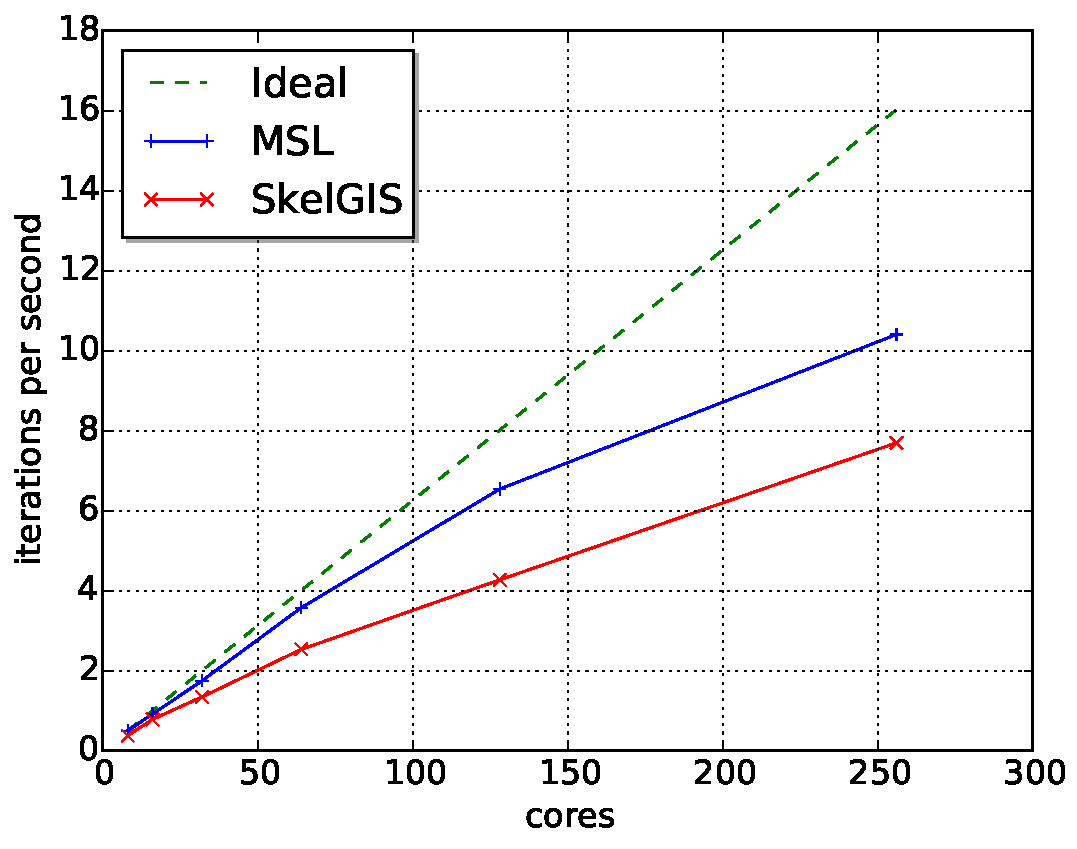
\includegraphics{./images/itpersec_5K_500.pdf}}
}
\hspace{5pt}
\subfloat[$10k \times 10k$ mesh, $500$ iterations\label{fig:speedup2}]{
\resizebox{5.5cm}{!}{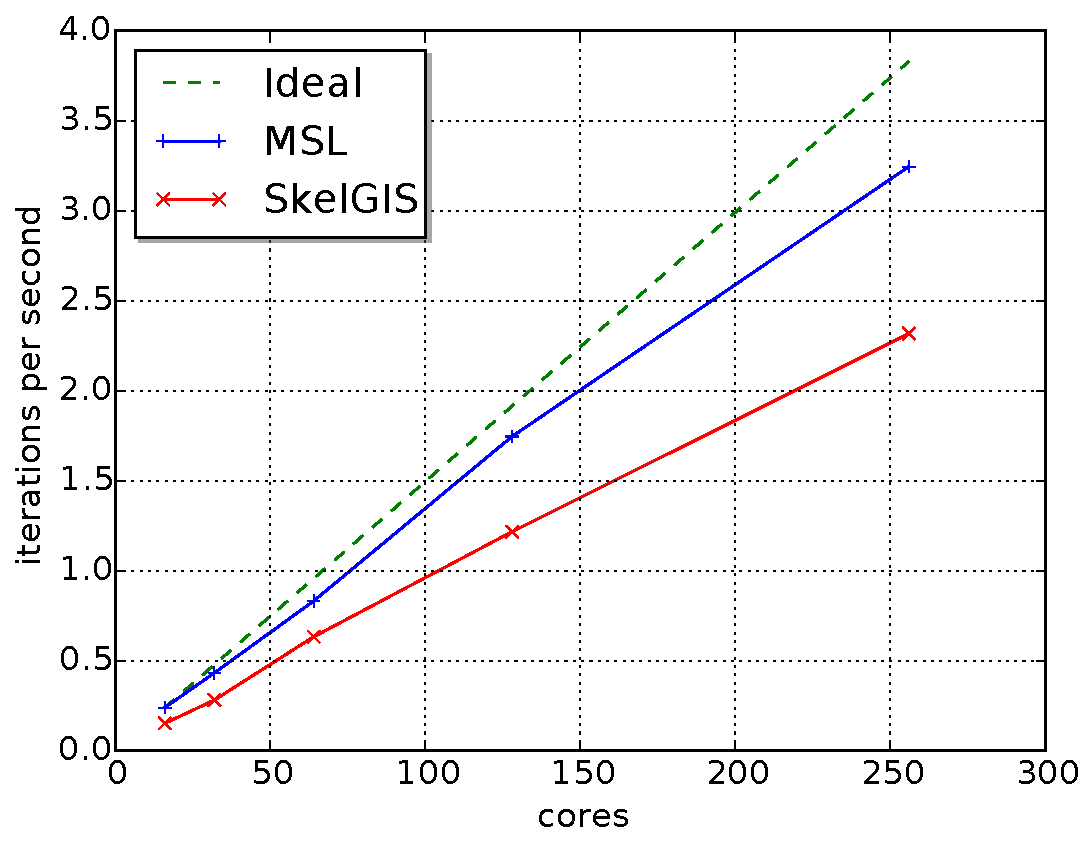
\includegraphics{./images/itpersec_10K_500.pdf}}
}
\hspace{5pt}
\subfloat[$10k \times 10k$ mesh, $2k$ iterations\label{fig:speedup3}]{
\resizebox{5.5cm}{!}{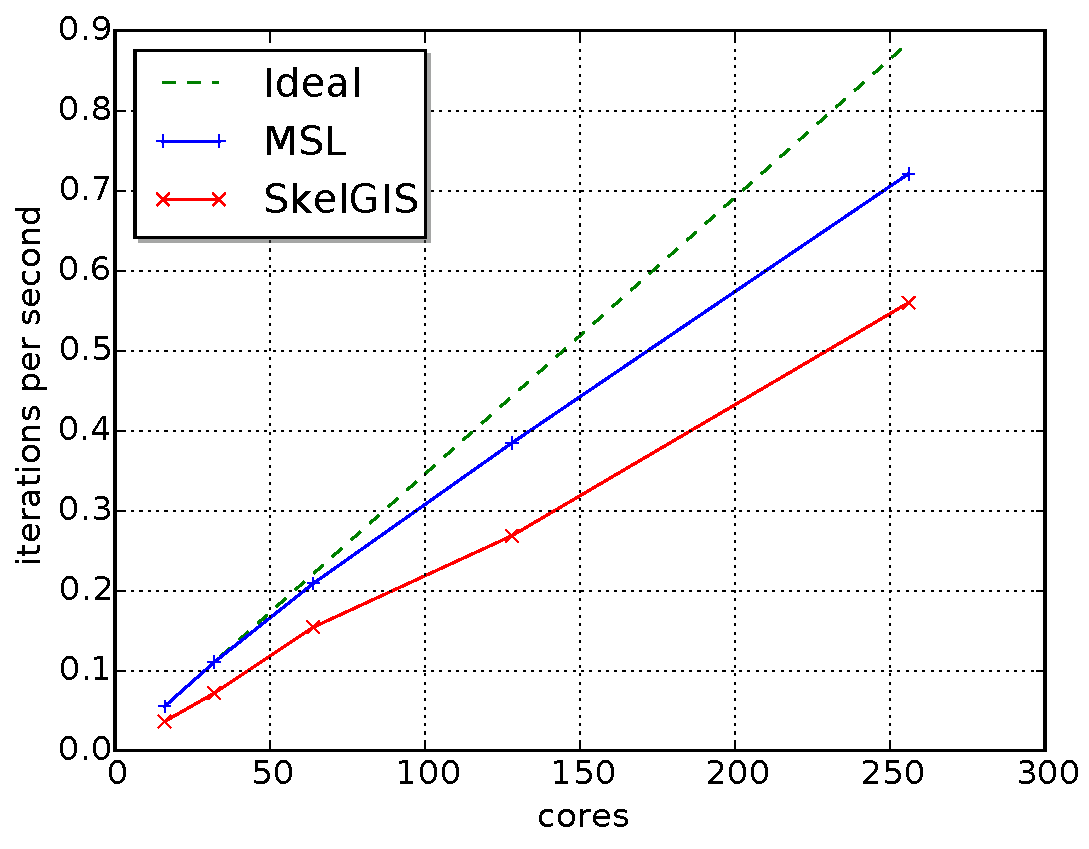
\includegraphics{./images/itpersec_10K_2K.pdf}}
}

\subfloat[$5k \times 5k$ mesh, $500$ iterations\label{fig:log21}]{
\resizebox{5.5cm}{!}{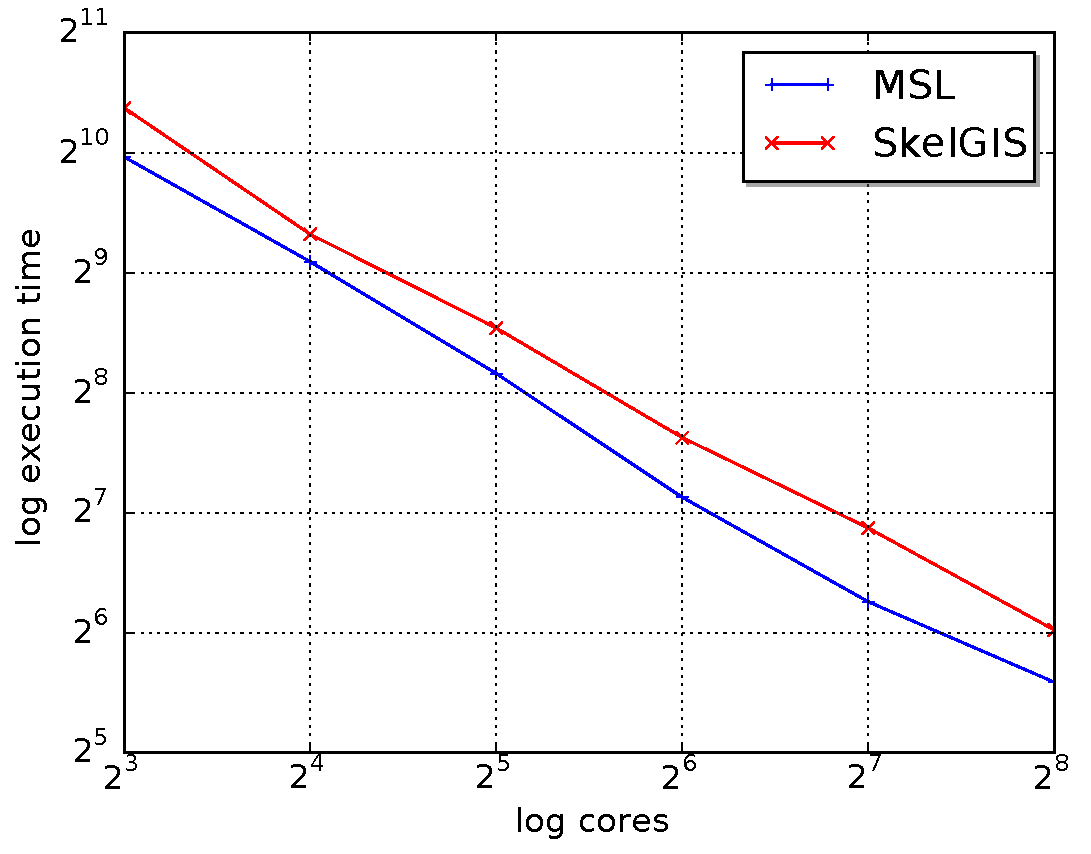
\includegraphics{./images/logtimes_5K_500.pdf}}
}
\hspace{5pt}
\subfloat[$10k \times 10k$ mesh, $500$ iterations\label{fig:log22}]{
\resizebox{5.5cm}{!}{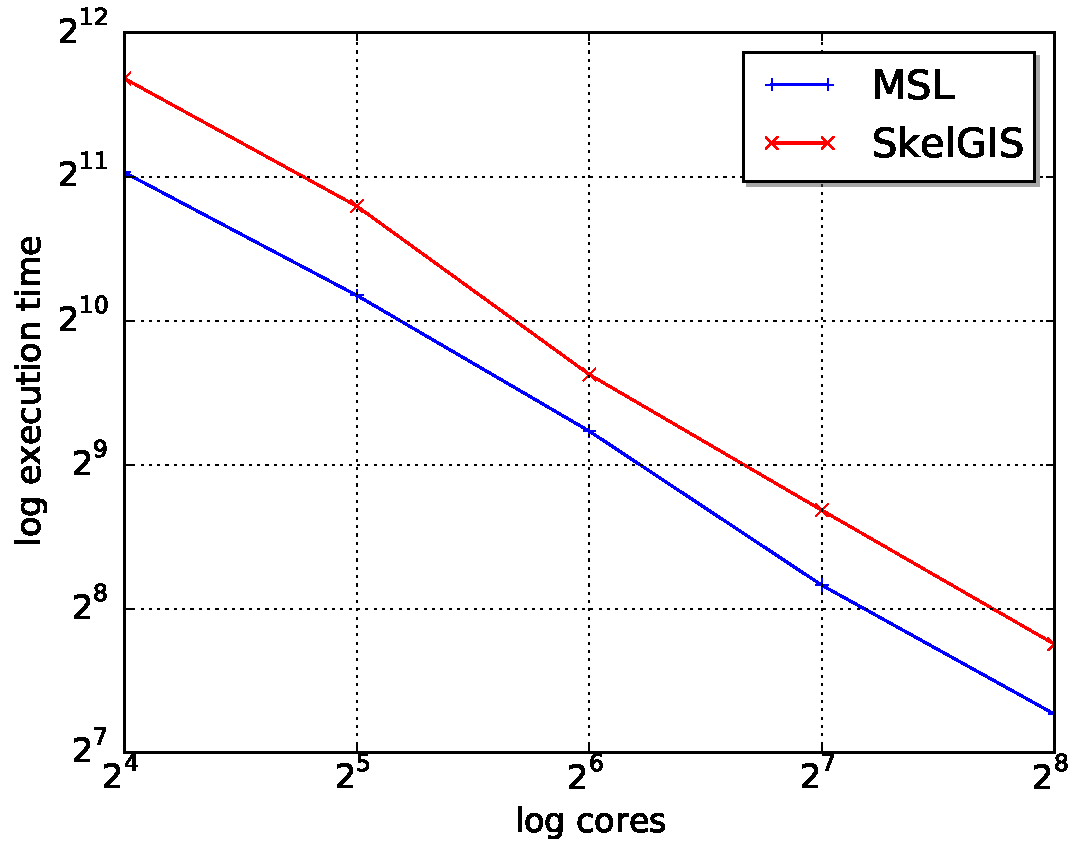
\includegraphics{./images/logtimes_10K_500.pdf}}
}
\hspace{5pt}
\subfloat[$10k \times 10k$ mesh, $2k$ iterations\label{fig:log23}]{
\resizebox{5.5cm}{!}{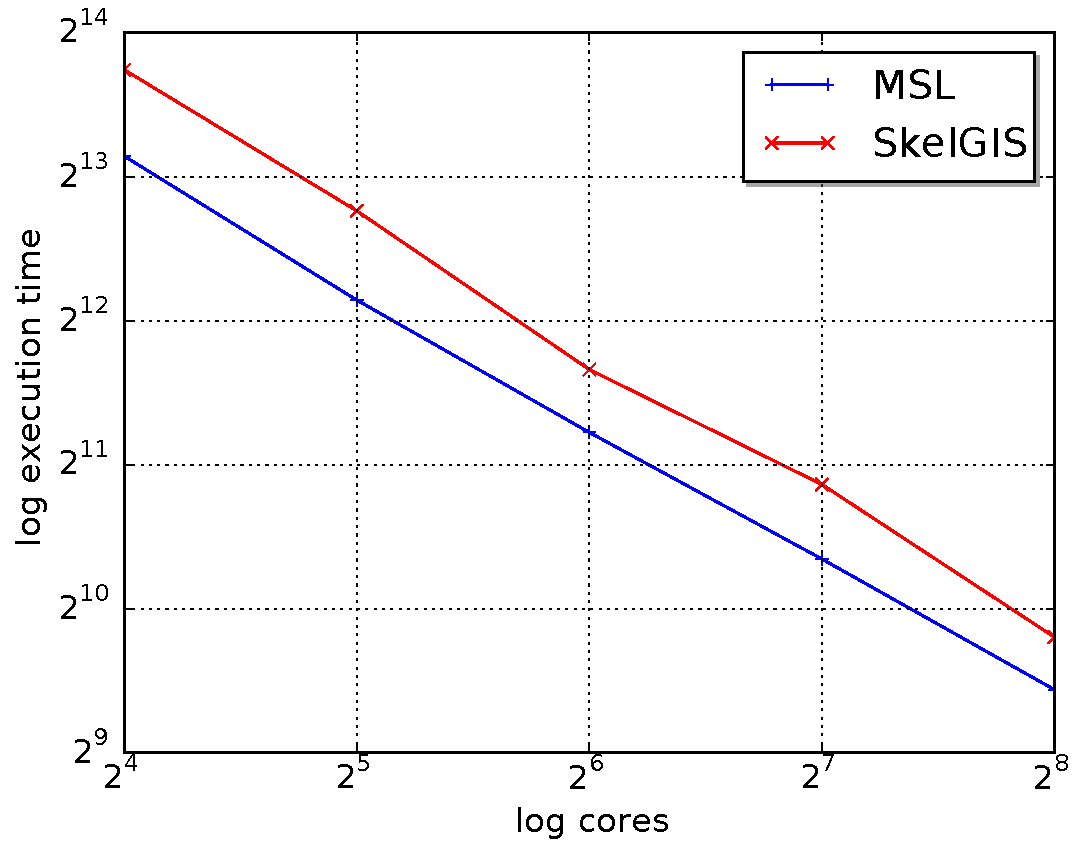
\includegraphics{./images/logtimes_10K_2K.pdf}}
}
\end{center}
\caption{The first line represents, for each experiment, the number of iteration computed per second for a given number of cores. The second line represents, for each experiment, the execution time for a given number of cores, using a logarithmic scale.}
\label{fig:perfs}
\end{figure*}

One can notice that, for the three different experiments, execution times of MSL, which itself uses the SkelGIS distributed data structure, are improved compared to a pure SkelGIS parallelization. This result can be explained by the automatic generation of the parallel component-based runtime. Actually, in a pure SkelGIS code, communications between processes are hidden from the user through specific interfaces called \emph{applicators}~\cite{CPE:CPE3494}. Using MSL, on the other hand, communications are directly managed by $SYNC$ components, which are automatically placed in the component-based runtime by MSCAC. Thus, no overhead is introduced to hide communications.

In addition to this, the scalability slope, shown by the number of iterations per second, is close to SkelGIS. This is an important result as the execution time of MSL is at the same time improved compared to SkelGIS. Actually, the less the execution time is, the less the scalability capacity is. Thus, these results confirm the result of~\cite{l2c} that using a component-based runtime does not damage performance of the back-end code. Finally, we notice that SkelGIS has proved its scalability on the Shallow water equations compared to an MPI parallelization~\cite{CPE:CPE3494}, that makes out performance results relevant. 
